\subsection{Structural evolution (H4, H5)}\label{sec:r-evolution}
\subsubsection{Growth, ageing and densification of the citation network (H4)}
\paragraph{Preferential attachment (H4a).}
The conditional attachment kernel $(k+1)^\alpha$ yields $\alpha=0.714$ with a descriptive
95\% year-bootstrap interval $[0.693,0.730]$ (\cref{fig:growth}a). Twenty P3a samples give
$0.0006\pm0.0051$ and the age-only control P3b gives $-0.6512\pm0.0053$
(\cref{fig:growth}b); the observed exponent exceeds all null values, corresponding to an
empirical one-sided probability of $1/21$ per comparison. The exponent remains positive
under time splits, degree offsets of 0.5 and 2, and a core subset of venues
(\cref{sec:r-robustness}). Sublinear degree preference is therefore supported within this
corpus beyond the age-only reference, without identifying a causal attachment mechanism.

\begin{figure*}[t]
\centering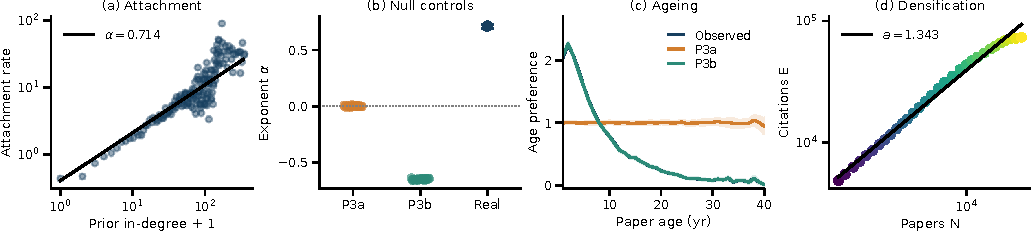
\includegraphics[width=\textwidth]{b_manuscript_growth.pdf}
\caption{CIT growth mechanisms. (a) Attachment rate by prior-degree class (classes with at
least five citations); the line shows the fitted exponent. (b) Exponents of 20 samples per
reference model and the observed exponent with its year-bootstrap interval. (c)
Exposure-adjusted age preference (null mean $\pm$ SD). (d) Cumulative edge count against
node count, 1990--2020.}
\label{fig:growth}
\end{figure*}

\paragraph{Ageing (H4b).}
A lognormal age kernel is preferred over exponential, power-law and uniform kernels
(\cref{tab:b-age-models}). The fitted parameters are $(\mu,\sigma)=(1.858,1.108)$,
corresponding to a scale $e^\mu$ of 6.41 years. The mean age of cited papers is 5.711
years, against $11.457\pm0.034$ under P3a and $5.717\pm0.018$ under the calibrated control
P3b (\cref{fig:growth}c). The lognormal kernel is preferred in all three publication
cohorts, although the tails of the most recent cohort remain censored. Age-independent
target choice is therefore rejected; the agreement of P3b follows from its calibration and
does not constitute independent confirmation.

\begin{table}[t]
\centering\small
\setlength{\tabcolsep}{4pt}
\begin{tabular*}{\columnwidth}{@{\extracolsep{\fill}}lrr@{}}
\toprule Age kernel & Parameters & $\Delta$AIC\\
\midrule
Lognormal & 2 & 0.0\\
Exponential & 1 & 537.8\\
Power-law & 1 & 9,360.5\\
Uniform & 0 & 41,796.7\\
\bottomrule
\end{tabular*}
\caption{CIT age-preference kernels fitted on identical observations. AIC selects among
the stated models and not among all possible ageing mechanisms.}
\label{tab:b-age-models}
\end{table}

\paragraph{Densification and diameter (H4c).}
For 1990--2020 the densification exponent is $a=1.343$ ($R^2=0.991$) with a descriptive
year-resampling interval $[1.288,1.406]$ (\cref{fig:growth}d). Densification is weaker in
2005--2020 ($a=1.065$) than in 1990--2004 ($a=1.455$). Here densification denotes
superlinear growth of the edge count and not increasing directed density. The effective
diameter of the largest weak component equals 6 hops in every year and is unchanged with
64 or 256 source nodes, so no shrinkage is detected at this resolution. Because P3 fixes
$N(t)$ and $E(t)$, it preserves $a$ by construction and cannot test densification.

\paragraph{Citation dynamics and prediction (H4d).}
For 500 full-history fits, the median WSB parameters are
$(\lambda,\mu,\sigma)=(2.717,0.834,1.238)$, with median RMSLE 0.074 and scaled-collapse RMSE
0.022; these are in-sample diagnostics. In the held-out task (\cref{tab:b-forecast}), WSB
predicts cumulative citations at age 15 with an MAE of 15.144, against 17.064 for linear
extrapolation. The paired difference (WSB minus linear) has a 95\% bootstrap interval of
$[-4.471,0.806]$ at age 15 and $[-4.764,8.128]$ for the 2020 total; both intervals contain
zero. The no-ageing baseline over-extrapolates by several orders of magnitude, so
outperforming it alone is a weak test. Forecast fits reach a parameter bound for 193 of 500
papers (38.6\%), although all optimizations report success; boundary solutions reflect limited
identifiability in short histories rather than optimizer failure. Compact descriptive fits
are thus supported, whereas a predictive advantage over linear extrapolation is not
established.

\begin{table}[t]
\centering\small
\setlength{\tabcolsep}{4pt}
\begin{tabular*}{\columnwidth}{@{\extracolsep{\fill}}llrr@{}}
\toprule Target & Model & MAE & RMSLE\\
\midrule
Age 15 & WSB & 15.144 & 0.601\\
 & Linear & 17.064 & 0.662\\
 & No-ageing PA & 27,588 & 4.601\\
\midrule
2020 & WSB & 28.016 & 0.778\\
 & Linear & 27.271 & 0.876\\
 & No-ageing PA & $2.79\!\times\!10^6$ & 7.000\\
\bottomrule
\end{tabular*}
\caption{Citation forecasts for 500 papers trained on years 1--5. Age 15 is the primary,
fixed-horizon target; the 2020 total is a secondary target with variable horizon.}
\label{tab:b-forecast}
\end{table}

\paragraph{Verdict on H4.}
Sublinear preferential attachment, age-dependent target choice and superlinear edge growth
are supported within this corpus, whereas diameter shrinkage and a forecast advantage of the
WSB model are not. All counts are restricted to the selected venues.

\subsubsection{Dynamic and static communities (H5)}
\paragraph{Primary school.}
Outside the midday break, snapshot communities closely match the classes (NMI
$\approx 0.85$--$0.95$), as does the static partition (six communities, NMI 0.86 with the
classes; \cref{fig:m4-ps}). Between approximately 12:00 and 14:00 on both days, the NMI with
the classes and with the static partition falls to $\approx 0.5$. Under P1 both curves remain
flat (class NMI $0.86\pm0.002$), so the decline is attributable to the timing of contacts
and not to the identity of the contacting pairs. Nor is it algorithmic noise: two Leiden runs
on the same window agree with NMI 0.98 on average. Averaged over the day, real snapshots agree
less with the static partition than P1 snapshots (0.72 against $0.94\pm0.003$).

\begin{figure*}[t]
\centering
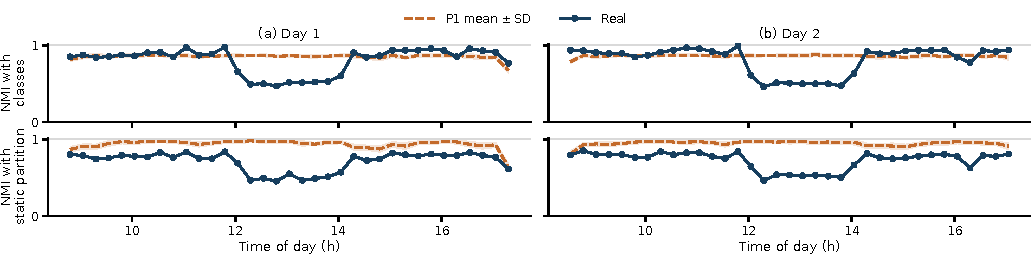
\includegraphics[width=\linewidth]{e_m4_ps_timeseries.pdf}
\caption{Snapshot communities in PS (15-min windows, $\gamma=1$): NMI with the classes (top)
and with the static partition (bottom). P1: mean $\pm$ SD of 20 samples.}
\label{fig:m4-ps}
\end{figure*}

\paragraph{CollegeMsg.}
Weekly snapshots agree only weakly with each other and with the static partition (NMI 0.52
and 0.34), and P1 yields similar values (0.42 and 0.32). Snapshots are sparse, with on
average 326 of 1,899 users active per week, and during the first two months two runs of
the algorithm on the same window agree only at NMI $\approx 0.65$--$0.7$. Where real and
null values differ, real snapshots resemble their predecessor more than randomized
snapshots do, which indicates persistent conversation groups rather than reorganisation.
This community-level result is distinct from the tie-level overlap of \cref{sec:r-activity}.

\paragraph{Sensitivity.}
The comparison was repeated for three window widths and three resolutions $\gamma$. In PS,
real snapshots agree less with the static partition than P1 snapshots in all nine settings
(differences between $-0.03$ and $-0.23$). In CM the difference remains within $\pm0.06$,
and within $\pm0.025$ except for 30-day windows with $\gamma=0.5$. The comparison with the
previous window is not robust in PS: at 15 and 60\,min real snapshots change more than P1
snapshots, whereas at 5\,min the order reverses, because a 5-min P1 snapshot is a small
random sample of the static graph. Larger $\gamma$ yields more and smaller communities
without changing these signs. Timestamp permutation spreads each node's events over the
whole period, so a P1 window contains almost all nodes (240 against 175 active nodes per
15-min PS window); part of the gap to the static partition therefore reflects which nodes
are active at a given time, in addition to which nodes interact. The midday decline of the
class NMI is unaffected, because it compares real snapshots with external labels.

\paragraph{Verdict on H5.}
H5 is supported for face-to-face contacts and not supported for online messages. In PS the
static partition recovers the classes but conceals the midday mixing, which P1 does not
reproduce. In CM the static partition summarises the weekly snapshots as well as it
summarises time-shuffled ones, and the snapshots are, if anything, more persistent than
random.
